\section{Coppertwait}
Coppertwait's rainfall models have been used for decades with a good deal of sucess. Although we will not dive deep into his methodology the following papers may be refferenced if one wishes too **ref all coppertwait papers**.

Over time, Coppertwait has improved and adjusted his model for varying applications. For example, in one of his more recent papers **ref 2010 paper**, Coppertwait has turned the discrete variable describing the type of storm into a continous one. This changes and developments, while interesting, are not the focus of our paper. Instead, we will focus on **ref 1994 paper** to understand the model at its simplicity and one may apply these ideas to a Hidden Markov Model. 

All of Coppertwaits models use a Neyman-Scott point processes to describe the arrival of Storms. The model itself can be described as follows:
\begin{itemize}
    \item The origin of each storm is a Poisson process in space-time
    \item Each storm is a circular region in two dimensional space with radii given by independent exponential random variables.
    \item Each storm generates a cluster of two dimensional circular rain cells with random duration, poistion and radius. 
    \item The duration of each cell is an exponential random variable.
    \item The intensity of each cell is a random exponential distributed but dependent on the type of cell. In **ref 1994** we have two cell types, light and heavy.
    \item Overall intensity at any point is given by the sum of overlaping intensities at the point in space and time.
\end{itemize}

The GNSRP Model, discussed in **ref paper 1994**, is a generalisation of the Neyman-Scott-Rectangular-Pulse (NSRP) Model with only one cell type. The key feature of the NSRP is that, in addition to those above, the distance from Cell origins to its Storm origin are independently exponentially distributed. Unlike other models that used and independent uniform distribution for this, NSRP accounted for the realistic effect that rainfall tends to be more intense near the center of the storm ** ref browning**.

\section{Grando - HMM Based Model}
\subsection{Model}
Grando extended on Coppertwait's ideas in **ref paper**. She completely removes the double disc structure and attempts to enclose the correlations within the larger Storm discs from Coppertwait in Hidden Markov States.

She defines her discrete time intensity process as follows:
For $n \geq 1$ and $x \in A$, where $A \subset \mathbb{R}^2$
\begin{equation}
    I_n(x) := \sum_{i=1}^{N^{(n)}} \sigma_i^{(n)} \mathbb{I}_{D(x_i^{(n)},R_i^{(n)})} (x)
\end{equation}
where:
\begin{itemize}
    \item $I_n(x)$ is the rain intensity
    \item $N^{(n)} \sim$ Pois($\lambda$) represents the number of rain discs generated
    \item $\sigma_i^{(n)} \sim$ Exp($\tau$) is a random variable providing the rain intensity
    \item  $D(x_i^{(n)},R_i^{(n)})$ is a rain disc with centre $x_i^{(n)} \sim$ Unif($A$) and radius $R_i^{(n)} \sim$ Exp($\xi$).
    \item $\mathbb{I}_{D(x_i^{(n)},R_i^{(n)})} (x)$ is an indicator function, equal to 1 if the current rain disc overlaps position $x$.
\end{itemize}

Parameters $\lambda$,$\xi$ and $\tau$ are taken to be fixed for each type of storm. In other words, for each hidden state of the HMM there is a unique $\lambda$,$\xi$ and $\tau$. Informally, the model has hidden states which determine the type of storm. This then dictates the values of the three above parameters, which in turn influence the intensity of rain observed.

Thus we arrive at the learning problem. Due to the added complexity of additional parameters we are unable to directly use methods for HMMs discussed earlier in the paper. Direct likelihood calculation is complex for HMMs alone, after we introduce these additional parameters it is not feasible. 

Given the model has $m$ states, we will have $m^2+4m$ unknown parameters, $m^2$ for the transition probabilities, $m$ for the intitial distribution and $m$ for each of $\lambda$,$\xi$ and $\tau$.  This is clearly a high-dimensional problem. To overcome this Grando fixes certain paramters in order to gain a better understanding of the remaining. She uses two methods; Nealder-Mead and Approximate Bayesian Computation. We will focus on the latter as it has provided superior results in her testing.

\subsection{Model Fitting}
We begin by trying to replicate Grando's results in order to establish a starting point. For ABC we require the prior distribution along with a summary statistic. Deriving the prior distribution is not a trivial problem. We not only have parameters for the HMM as well as parameters for the observations but have to  extract both from only the intensity values. 

Grando determines that even without the HMM parameters, the problem is high dimensional (3$m$ paramters). Due to this she decides to fix all HMM paramters to uniform(0,1) for each test, whilst insuring the transition matrix is stochastic through normalization of rows. She believes that this will allow her to retrieve close approximations of all $\lambda$,$\xi$ and $\tau$ from the data, which she can then use to calculate the HMM paramters. 

For each simulation she will generate a new value for all $\lambda$,$\xi$ and $\tau$. Then plot the summary statistic against the values for each and then find areas of high concentration to decide what a sutiable approximation for the true value of each is. Here she is setting her ABC tolerance to $\infty$ and then manually narrowing her range through the graph.

Grando picks values for each paramter using the uniform distribution between preset values. She says "This technique is purely heuristic and it is only aimed to explore the problem, as decisions made are completely arbitrary.". Theoretically we could pick any values for  but for consistency we will match the values she has used.  

She decides to use the mean intensity as her summary statistic for ABC. She calculates this for both the simulated and given data. She then calculates the normalised Euclidean distance between the two as her metric for model performance.


\section{Numerical Results}
We will be using the same algorithm, same data and same parameters as Grando to ensure consistency. Our data measures rainfall across 30 sites in Germany over the period from 1st of january 1931 to 31st December 2000. Co-ordinate data for each site is also given in an additional file. These are labeled as Easting and Northing. 

Grando fixes $m$=3, allowing for a low, medium and high state for rainfall. This gives us 21 unknown parameters of which we are attempting to estimate 9.

All programs have been run on the personal desktop (AMD Ryzen™ 9 3900X with 12 Cores and 24 Threads running from 3.8GHz up to 4.6GHz) using C++20.

\subsection{Code}

To ensure validity of results, we wanted to run multiple tests. Grando's code was written in R and required multiple hours to produce a result. To improve on this we have rewritten the program in C++ and used Python on Jupyter Notebooks for analysis.

Data preperation took place in excel. For simplicity in importing into C++, the data needed to be configured in a particular way. This is described throughly in the notes given with the code. 

C++ was used for the actual simulation as this was the slowest part of Grandos algorithm. Many parameters have been hardcoded. This is to allow for efficiency and can later be altered if needed. Notes on mininpulating the code can be found **reference to later**. Multi-threading has been used for further reduction in run-time. Admittdely the code can be further parallised but in its current state it is acceptable; run times of under 5 minutes. 

Analysis was done using Python in Jupyter Notebooks. The C++ program created multiple CSV files as output and these were taken as input for analysis. 

\subsection{Analysis - Nine Parameter Estimation}

We begin with using ABC to estimate all parameters, found on pages 75-76 **Grando ref**. The parameters are picked as follows:

\begin{itemize}
    \item $\lambda_1 \sim \text{Unif(5,15)}$, $\lambda_2 \sim \text{Unif(16,25)}$ and $\lambda_3 \sim \text{Unif(26,35)}$
    \item $\xi_1 \sim \text{Unif(0.03,0.07)}$, $\xi_2 \sim \text{Unif(0.008,0.02)}$ and $\xi_3 \sim \text{Unif(0.001,0.007)}$
    \item $\tau_1 \sim \text{Unif(0.8,1.4)}$, $\tau_2 \sim \text{Unif(0.3,0.7)}$ and $\tau_3 \sim \text{Unif(0.07,0.2)}$
\end{itemize}

For each simulation we generate data for 365x5 days and calculate the normalised Euclidean distance between the mean of these and the mean of the whole given dataset. Due to random sampling we attempt to find estimates for all 9 parameters simultaneously. We completed 200 iterations on the personal desktop in 42.2841 seconds.

\begin{figure}
    \begin{subfigure}{.5\textwidth}
      \centering
      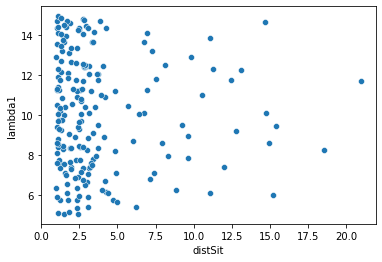
\includegraphics[width=\linewidth]{./AllParam/lambda_1.png}
      \caption{$\lambda_1$ }
      \label{allp:lambda1}
    \end{subfigure}
    \begin{subfigure}{.5\textwidth}
      \centering
      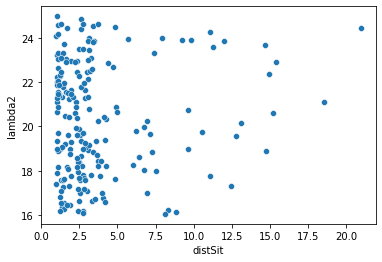
\includegraphics[width=\linewidth]{./AllParam/lambda_2.png}
      \caption{$\lambda_2$ }
      \label{allp:lambda2}
    \end{subfigure}
    \begin{subfigure}{.5\textwidth}
        \centering
        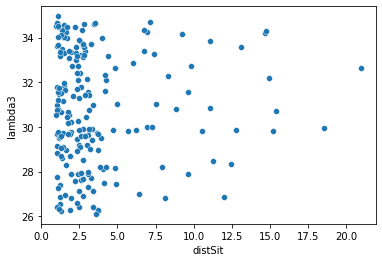
\includegraphics[width=\linewidth]{./AllParam/lambda_3.png}
        \caption{$\lambda_3$ }
        \label{allp:lambda3}
    \end{subfigure}
    \begin{subfigure}{.5\textwidth} 
        \centering
        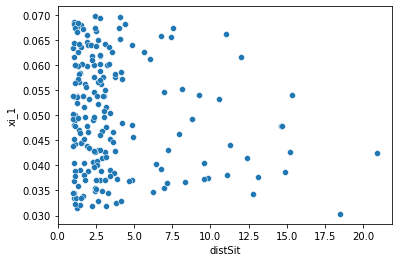
\includegraphics[width=\linewidth]{./AllParam/xi_1.png}
        \caption{$\xi_1$ }
        \label{allp:xi1}
    \end{subfigure}
    \begin{subfigure}{.5\textwidth}
        \centering
        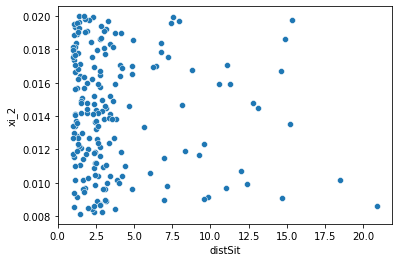
\includegraphics[width=\linewidth]{./AllParam/xi_2.png}
        \caption{$\xi_2$ }
        \label{allp:xi2}
    \end{subfigure}
    \begin{subfigure}{.5\textwidth}
        \centering
        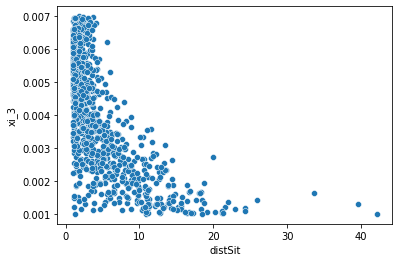
\includegraphics[width=\linewidth]{./AllParam/xi_3.png}
        \caption{$\xi_3$ }
        \label{allp:xi3}
    \end{subfigure}
    \begin{subfigure}{.5\textwidth}
        \centering
        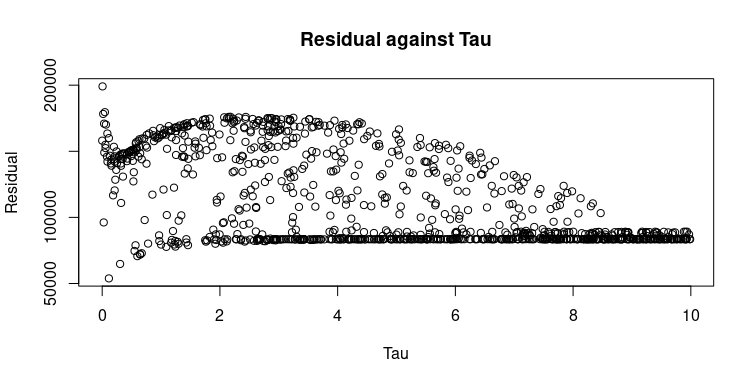
\includegraphics[width=\linewidth]{./AllParam/tau_1.png}
        \caption{$\tau_1$ }
        \label{allp:tau1}
    \end{subfigure}
    \begin{subfigure}{.5\textwidth}  
        \centering
        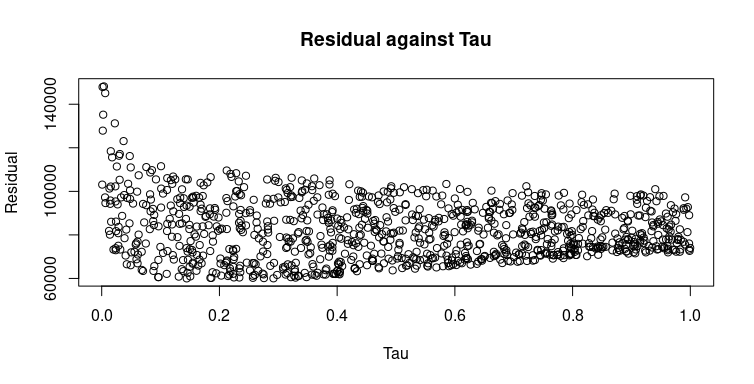
\includegraphics[width=\linewidth]{./AllParam/tau_2.png}
        \caption{$\tau_2$ }
        \label{allp:tau2}
    \end{subfigure}

    \centering
    \begin{subfigure}{.5\textwidth}
        \centering
        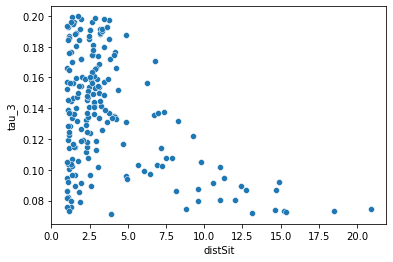
\includegraphics[width=\linewidth]{./AllParam/tau_3.png}
        \caption{$\tau_3$ }
        \label{allp:tau3}
    \end{subfigure}

      \caption{Parameter values plotted against corresponding normalised Euclidean Distance between simulation and data means.}
      \label{allp}
\end{figure}
    
The results show ABC on nine parameters was not successful. Figure **ref** show for all parameters an extremly unifrom scatter suggesting the posterior distribution is still uniform in a neighbourhood of the true parameters. This is an exact match to Grando's results. 

\subsection{Analysis - Three Parameter Estimation}
Grando then decides to perform ABC on a subset of our nine parameters. She claims choosing only  $\lambda_i$,only $\xi_i$ or only $\tau_i$ does not yield better outcomes. She then goes on to test for only $\lambda_3$,$\xi_3$ and $\tau_3$, fixing all other parameters to abritary values. Once again, for consistency we choose values to match those of Grando.

\begin{itemize}
    \item $\lambda_1 = 10$, $\lambda_2 = 20$ and $\lambda_3 =30$
    \item $\xi_1 = 0.05$, $\xi_2 = 0.01 $ and $\lambda_3 =0.005$
    \item $\tau_1 =1.1$, $\tau_2 = 0.5$ and $\tau_3 =0.1$
\end{itemize}

For each test we require three simulations. When computing for $\lambda_3$ we change its value from 30 to $\lambda_3 \sim \text{Unif(26,35)}$. Similarly, when computing for $\xi_3$, we change its value to $\xi_3 \sim \text{Unif(0.001,0.007)}$ and when computing for $\tau_3$ we change its value to $\tau_3 \sim \text{Unif(0.07,0.2)}$. At any given time there is one random variable between our nine that we are testing. For efficiency we process this over multiple threads. We completed 100 iterations and ran 5 attempts on the personal desktop. Attempt time ranged between 152.725 in to 199.386 seconds.

\begin{figure}
    \begin{subfigure}{.5\textwidth}
      \centering
      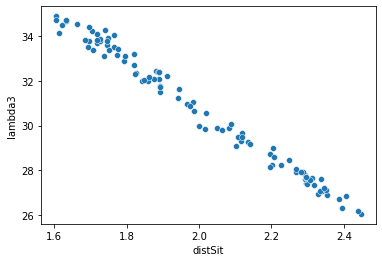
\includegraphics[width=\linewidth]{./SingleParam/lambda_3_1.png}
      \caption{Attempt 1}
      \label{singlelam:1}
    \end{subfigure}
    \begin{subfigure}{.5\textwidth}
      \centering
      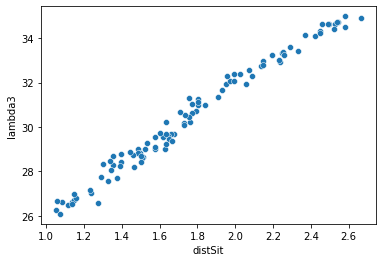
\includegraphics[width=\linewidth]{./SingleParam/lambda_3_2.png}
      \caption{Attempt 2}
      \label{singlelam:2}
    \end{subfigure}
    \begin{subfigure}{.5\textwidth}
        \centering
        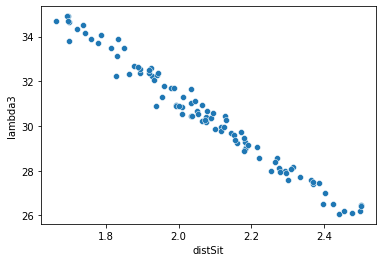
\includegraphics[width=\linewidth]{./SingleParam/lambda_3_3.png}
        \caption{Attempt 3}
        \label{singlelam:3}
    \end{subfigure}
    \begin{subfigure}{.5\textwidth} 
        \centering
        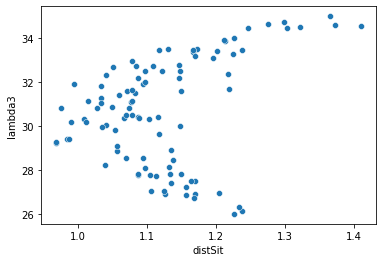
\includegraphics[width=\linewidth]{./SingleParam/lambda_3_4.png}
        \caption{Attempt 4}
        \label{singlelam:4}
    \end{subfigure}
    \begin{subfigure}{.5\textwidth}
        \centering
        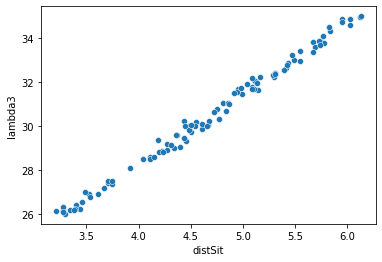
\includegraphics[width=\linewidth]{./SingleParam/lambda_3_5.png}
        \caption{Attempt 5}
        \label{singlelam:5}
    \end{subfigure}

    \caption{$\lambda_3$ values plotted against corresponding normalised Euclidean Distance between simulation and data means for 5 attempts.}
    \label{singlelam}
\end{figure}

\begin{figure}
    \begin{subfigure}{.5\textwidth}
      \centering
      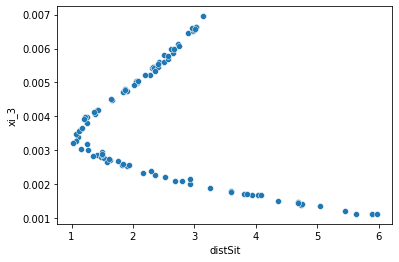
\includegraphics[width=\linewidth]{./SingleParam/xi_3_1.png}
      \caption{Attempt 1}
      \label{singlexi:1}
    \end{subfigure}
    \begin{subfigure}{.5\textwidth}
      \centering
      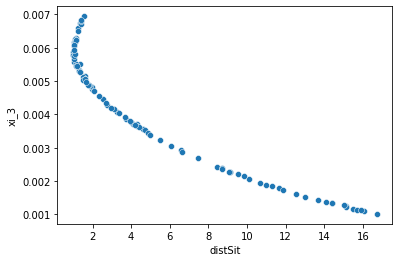
\includegraphics[width=\linewidth]{./SingleParam/xi_3_2.png}
      \caption{Attempt 2}
      \label{singlexi:2}
    \end{subfigure}
    \begin{subfigure}{.5\textwidth}
        \centering
        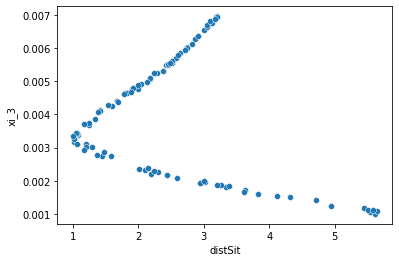
\includegraphics[width=\linewidth]{./SingleParam/xi_3_3.png}
        \caption{Attempt 3}
        \label{singlexi:3}
    \end{subfigure}
    \begin{subfigure}{.5\textwidth} 
        \centering
        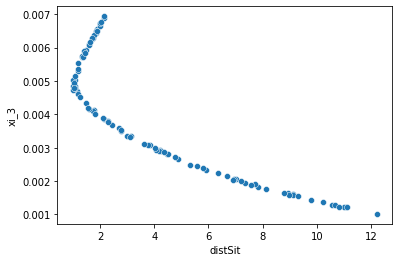
\includegraphics[width=\linewidth]{./SingleParam/xi_3_4.png}
        \caption{Attempt 4}
        \label{singlexi:4}
    \end{subfigure}
    \begin{subfigure}{.5\textwidth}
        \centering
        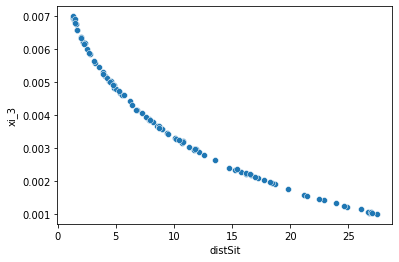
\includegraphics[width=\linewidth]{./SingleParam/xi_3_5.png}
        \caption{Attempt 5}
        \label{singlexi:5}
    \end{subfigure}

    \caption{$\xi_3$ values plotted against corresponding normalised Euclidean Distance between simulation and data means for 5 attempts.}
    \label{singlexi}
\end{figure}

\begin{figure}
    \begin{subfigure}{.5\textwidth}
      \centering
      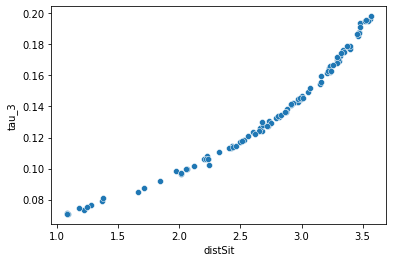
\includegraphics[width=\linewidth]{./SingleParam/tau_3_1.png}
      \caption{Attempt 1}
      \label{singletau:1}
    \end{subfigure}
    \begin{subfigure}{.5\textwidth}
      \centering
      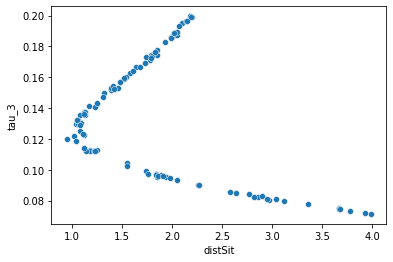
\includegraphics[width=\linewidth]{./SingleParam/tau_3_2.png}
      \caption{Attempt 2}
      \label{singletau:2}
    \end{subfigure}
    \begin{subfigure}{.5\textwidth}
        \centering
        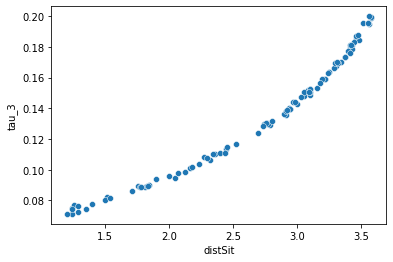
\includegraphics[width=\linewidth]{./SingleParam/tau_3_3.png}
        \caption{Attempt 3}
        \label{singletau:3}
    \end{subfigure}
    \begin{subfigure}{.5\textwidth} 
        \centering
        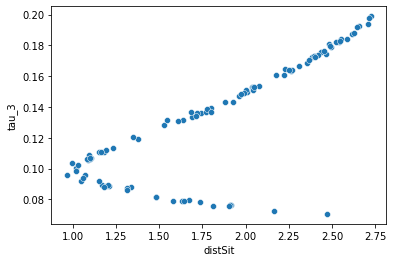
\includegraphics[width=\linewidth]{./SingleParam/tau_3_4.png}
        \caption{Attempt 4}
        \label{singletau:4}
    \end{subfigure}
    \begin{subfigure}{.5\textwidth}
        \centering
        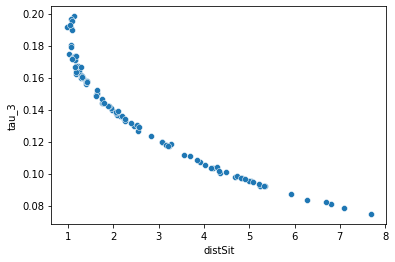
\includegraphics[width=\linewidth]{./SingleParam/tau_3_5.png}
        \caption{Attempt 5}
        \label{singletau:5}
    \end{subfigure}

    \caption{$\tau_3$ values plotted against corresponding normalised Euclidean Distance between simulation and data means for 5 attempts.}
    \label{singletau}
\end{figure}

\section{High Dimenstional Parameter Estimation}